\clearpage

\section{MQAM Receiver}

\begin{tcolorbox}	
	\begin{tabular}{p{2.75cm} p{0.2cm} p{10.5cm}} 	
		\textbf{Header File}   &:& m\_qam\_receiver.h \\
		\textbf{Source File}   &:& m\_qam\_receiver.cpp \\
	\end{tabular}
\end{tcolorbox}

\paragraph{Warning:}\textit{homodyne\_receiver} is not recommended. Use \textit{m\_qam\_homodyne\_receiver} instead.
\newline

This block of code simulates the reception and demodulation of an optical signal (which is the input signal of the system) outputing a binary signal. A simplified schematic representation of this block is shown in figure \ref{MQAM_receiver_block_diagram_simple}.

\begin{figure}[h]
	\centering
	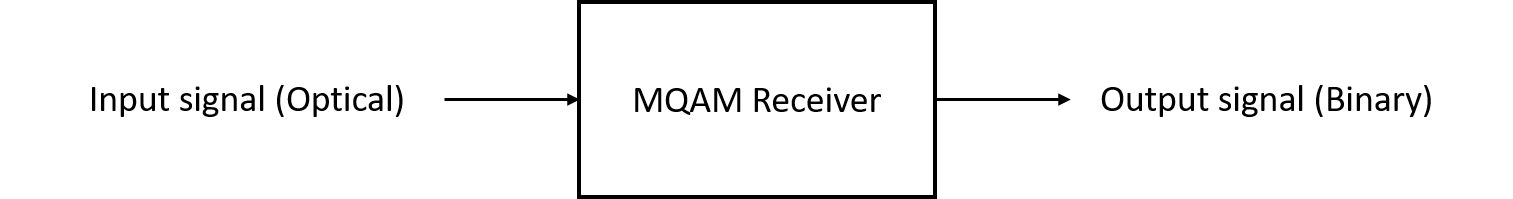
\includegraphics[width=0.8\textwidth]{../lib/homodyne_receiver/figures/MQAM_receiver_block_diagram_simple}
	\caption{Basic configuration of the MQAM receiver}\label{MQAM_receiver_block_diagram_simple}
\end{figure}

\subsection*{Functional description}

This block accepts one optical input signal and outputs one binary signal that corresponds to the M-QAM demodulation of the input signal. It is a complex block (as it can be seen from figure \ref{MQAM_receiver_block_diagram}) of code made up of several simpler blocks whose description can be found in the \textit{lib} repository.

In can also be seen from figure \ref{MQAM_receiver_block_diagram} that there's an extra internal (generated inside the homodyne receiver block) input signal generated by the \textit{Clock}. This block is used to provide the sampling frequency to the \textit{Sampler}.


\begin{figure}[h]
	\centering
	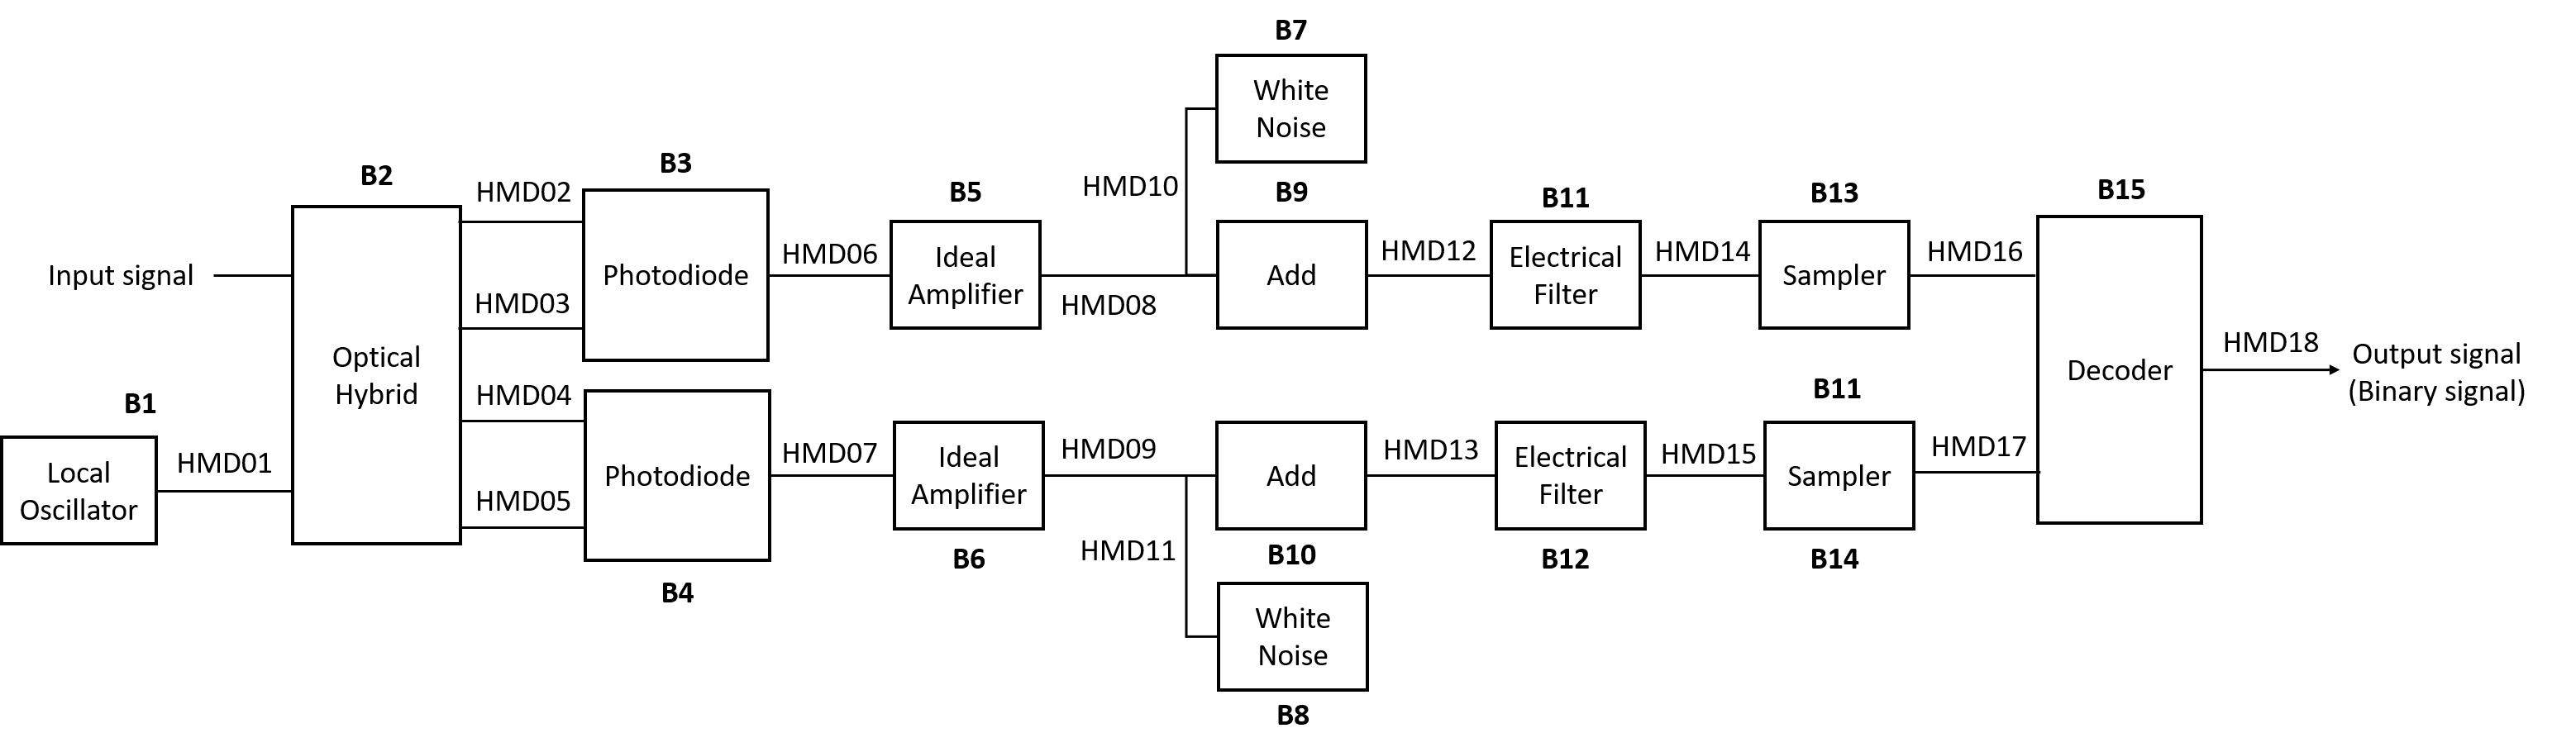
\includegraphics[width=\textwidth]{../lib/homodyne_receiver/figures/MQAM_receiver_block_diagram_20180206.png}
	\caption{Schematic representation of the block homodyne receiver.}\label{MQAM_receiver_block_diagram}
\end{figure}

\subsection*{Input parameters}

This block has some input parameters that can be manipulated by the user in order oto change the basic configuration of the receiver. Each parameter has associated a function that allows for its change. In the following table (table~\ref{table}) the input parameters and corresponding functions are summarized.

\begin{table}[h]
	\begin{center}
		\begin{tabular}{| m{3,2cm} | m{6,2cm} |  m{2,2cm} | m{4cm} | }
			\hline
			\textbf{Input parameters} & \textbf{Function} & \textbf{Type} & \textbf{Accepted values} \\ \hline
			IQ amplitudes & setIqAmplitudes & Vector of coordinate points in the I-Q plane & \textbf{Example} for a 4-QAM mapping: \{ \{ 1.0, 1.0 \}, \{ -1.0, 1.0 \}, \{ -1.0, -1.0 \}, \{ 1.0, -1.0 \} \} \\ \hline
			Local oscillator power (in dBm) & setLocalOscillatorOpticalPower\_dBm & double(t\_real) & Any double greater than zero\\ \hline
			Local oscillator phase & setLocalOscillatorPhase & double(t\_real) & Any double greater than zero\\ \hline
			Responsivity of the photodiodes & setResponsivity & double(t\_real) &$\in$ [0,1] \\ \hline
			Amplification (of the TI amplifier) & setAmplification & double(t\_real) & Positive real number\\ \hline
			Noise amplitude (introduced by the TI amplifier) & setNoiseAmplitude & double(t\_real) & Real number greater than zero \\ \hline
			Samples to skipe & setSamplesToSkip & int(t\_integer) &  \\ \hline
			Save internal signals & setSaveInternalSignals & bool & True or False\\ \hline
			Sampling period & setSamplingPeriod & double & Given by \textit{symbolPeriod}/\textit{samplesPerSymbol}\\
			\hline
		\end{tabular}
		\caption{List of input parameters of the block MQAM receiver} \label{table}
	\end{center}
\end{table}

\pagebreak

\subsection*{Methods}

HomodyneReceiver(vector$<$Signal *$>$ \&inputSignal, vector$<$Signal *$>$ \&outputSignal) (\textbf{constructor})
\bigbreak
void setIqAmplitudes(vector$<$t\_iqValues$>$ iqAmplitudesValues)
\bigbreak
vector$<$t\_iqValues$>$ const getIqAmplitudes(void)
\bigbreak
void setLocalOscillatorSamplingPeriod(double sPeriod)
\bigbreak
void setLocalOscillatorOpticalPower(double opticalPower)
\bigbreak
void setLocalOscillatorOpticalPower\_dBm(double opticalPower\_dBm)
\bigbreak
void setLocalOscillatorPhase(double lOscillatorPhase)
\bigbreak
void setLocalOscillatorOpticalWavelength(double lOscillatorWavelength)
\bigbreak
void setSamplingPeriod(double sPeriod)
\bigbreak
void  setResponsivity(t\_real Responsivity)
\bigbreak
void setAmplification(t\_real Amplification)
\bigbreak
void setNoiseAmplitude(t\_real NoiseAmplitude)
\bigbreak
void setImpulseResponseTimeLength(int impResponseTimeLength)
\bigbreak
void setFilterType(PulseShaperFilter fType)
\bigbreak
void setRollOffFactor(double rOffFactor)
\bigbreak
void setClockPeriod(double per)
\bigbreak
void setSamplesToSkip(int sToSkip)

\pagebreak

\subsection*{Input Signals}

\subparagraph*{Number:} 1

\subparagraph*{Type:} Optical signal

\subsection*{Output Signals}

\subparagraph*{Number:} 1

\subparagraph*{Type:} Binary signal

\subsection*{Example}

\subsection*{Sugestions for future improvement}
